%%%%%%%%%%%%%%%%%%%%%%%%%%%%%%%%%%%%%%%%%
% FRI Data Science_report LaTeX Template
% Version 1.0 (28/1/2020)
%
% Jure Demšar (jure.demsar@fri.uni-lj.si)
%
% Based on MicromouseSymp article template by:
% Mathias Legrand (legrand.mathias@gmail.com)
% With extensive modifications by:
% Antonio Valente (antonio.luis.valente@gmail.com)
%
% License:
% CC BY-NC-SA 3.0 (http://creativecommons.org/licenses/by-nc-sa/3.0/)
%
%%%%%%%%%%%%%%%%%%%%%%%%%%%%%%%%%%%%%%%%%


%----------------------------------------------------------------------------------------
%	PACKAGES AND OTHER DOCUMENT CONFIGURATIONS
%----------------------------------------------------------------------------------------
\documentclass[fleqn,moreauthors,10pt]{ds_report}
\usepackage[english]{babel}

\graphicspath{{fig/}}




%----------------------------------------------------------------------------------------
%	ARTICLE INFORMATION
%----------------------------------------------------------------------------------------

% Header
\JournalInfo{FRI Data Science Project Competition 2020}

% Interim or final report
\Archive{Final report}
%\Archive{Final report}

% Article title
\PaperTitle{How good is my plot?}

% Authors (student competitors) and their info
\Authors{Maruša Oražem, Urša Zrimšek, Andrej Hafner}

% Advisors
\affiliation{\textit{Advisors: Assoc. Prof. dr. Erik Štrumbelj , Assoc. Prof. dr. Tomaž Curk}}

% Keywords
\Keywords{visualizations, plots, quality perception}
\newcommand{\keywordname}{Keywords}


%----------------------------------------------------------------------------------------
%	ABSTRACT
%----------------------------------------------------------------------------------------

\Abstract{
Statistical plots are an essential tool for visual presentation of information, but their quality is often questionable. In order to determine which plot properties determine its quality, we construct a dataset of statistical plots obtained from student theses. We utilize the crowdsourcing platform Amazon Mechanical Turk for plot quality evaluation through pairwise plot comparisons. And we fine-tune convolutional neural networks and use them to extract image embeddings to predict plot quality. We are unable to achieve good predictive quality, which we suspect is due to poor data quality or insufficient amount of labeled data.
}

%----------------------------------------------------------------------------------------

\begin{document}

% Makes all text pages the same height
\flushbottom

% Print the title and abstract box
\maketitle

% Removes page numbering from the first page
\thispagestyle{empty}

%----------------------------------------------------------------------------------------
%	ARTICLE CONTENTS
%----------------------------------------------------------------------------------------

\section*{Introduction}
Statistical plots are one of the basic tools, which a scientist can use to convey information. They are used and abused in many scientific works, and are unfortunately often not of a good quality. Therefore, the goal of our project is to develop a model that can find out what are the properties of a high quality plot. When answering this question, we will focus on the visual aspect, because it simplifies our task and enables us to use deep learning techniques. With such approach we lose a very important part of the plot analysis -- how well it conveys information that it was intended for. But if we would want to include that in our research, it would be much more complicated, because we would need to have a deep understanding of the context and the data that was use for plot generation.

Code together with additional visualizations and examples is available in the Github \href{https://github.com/AndrejHafner/how-good-is-my-plot}{repository}.
% We start with the description of best practices when creating a plot. Next, we take a look at our dataset acquisition process and finish off with our plans for the future.

%------------------------------------------------

% \section*{Methods}
% Do we need this?

%------------------------------------------------
\section*{What makes a good plot?}
The biggest question we have to answer is, what makes a good plot? To get an overview on that, let's summarize the parts of the article \emph{Testing statistical Charts: What makes a Good Graph?} \cite{Whatmakesagoodplot}, that we can (at least implicitly) use in our approach of evaluating the plot's quality.

The main goal of statistical plots is to effectively and accurately present the data. Any additional enhancement on the plot should contribute to that aim. Here are some things that are considered to be current best practices.
Some of the important cognitive principles that the authors list are proximity of important things on the plots, similarity of groups, similar items should be in the common region, number of items that the human working memory can process and a hierarchy of what plot properties are easily compared.
% \begin{itemize}[noitemsep]
%     \item \textbf{Proximity}.
%     This principle tells us, that we need to put things we want to compare closer together, just the opposite for the less important things.
%     \item \textbf{Similarity}.
%     This principle tells us to group together things that somehow belong to the same group. We could do that with the same color or same shape.
%     \item \textbf{Common region}.
%     This principle suggests that elements that are contained in a common region, belong together.
%     \item \textbf{Working memory}.
%     This tells us about the limitation of our working memory. In general, we can not process more than $7 (\pm 2)$ items.
%     \item \textbf{Change blindness}.
%     This principle talks about the fact, that it is difficult to detect changes on a similar object.
%     \item \textbf{Ease of comparison}.
%     Some things are easier to compare than others. If things can be compared in a way that is higher in the following hierarchy, it should be done that way:
%     \begin{enumerate}[noitemsep]
%         \item position (common scale),
%         \item position (nonaligned scale),
%         \item length, direction, angle, slope,
%         \item area,
%         \item volume, density, curvature,
%         \item shading, color saturation, color hue,
%         \item discriminable shape,
%         \item indiscriminable shape.
%     \end{enumerate}
% \end{itemize}

It was shown that aesthetics used in plots can change how the data is read. A very important thing we need to consider is color. Color can change everything. Like we already stated, elements of the same group should have the same color. But what is that color? Color should be chosen to best match the data and plot type. If we are trying to show magnitude, we should use a univariate color scheme. On the other hand, if we want to show the data that differ in sign, we should use a double-ended color scale. If possible, we should keep the number of hues to a minimum, we should transit through neutral color, such as white when utilizing a gradient. These properties are a generalization of what is common in our perception, each person still has their own special preferences, therefore we'll utilize a crowdsourcing platform to acquire relevant data.

%------------------------------------------------
\section*{Getting the data}
The first task was to get the statistical plots to work with. We have chosen 7 different plot types -- box plot, line plot, bar plot, histogram, pie chart, scatter plot and violin plot. From \emph{Repository of the University of Ljubljana} \cite{repositoryUL} we downloaded bachelor's, master's and doctoral theses and extracted all images from them. For the extraction we used \href{https://github.com/pymupdf/PyMuPDF}{PyMuPDF} library. In order to filter the plots from the rest of the images, we first had to train a classifier. For training we scrapped plots from Google, Bing, and DuckDuckGo image search results, since they mostly return correct plot images. We manually filtered them and got approximately 400 images for each class.

%-----------------------------------------------
\section*{Classification model}
We used those images to train a convolutional neural network (CNN) to help us with the classification of images from student theses. The majority of images extracted from PDF-s were not plots, so we added the eight class called \texttt{not\_plot}. For its training set, we used 400 randomly selected images, extracted from the FRI bachelor's theses, from which we deleted any image that represented a plot.

Since our train dataset is small, we needed a pretrained network. We used the ResNet101 residual neural network, which has 101 layers and was trained on more than a million images of 1000 classesfrom ImageNet. A pretrained CNN is already good at recognizing representative shapes, we just need to fine-tune it to be able to separate between the classes we are interested in. We deleted the last layer and replaced it with a fully connected layer with 8 neurons, each representing one of our classes. Then we used Google Colab to do 50 epochs of training on our dataset, using Adam optimizer together with cross-entropy loss. We validated it in each epoch and saved the model that had the lowest loss on the validation set.

After the first iteration of training, we classified the first 2000 images from FRI bachelor's theses and sorted them into 3 groups -- those for which the model returned more than $99\%$ probability for the predicted class, those for which it returned more than $90\%$ and those for which it returned less. We then handpicked all incorrectly classified images from there, and also those correctly classified, that the model wasn't sure about, and added them to the training set. On figure \ref{wrong phase1} we can see some examples.

\begin{figure}[h]
	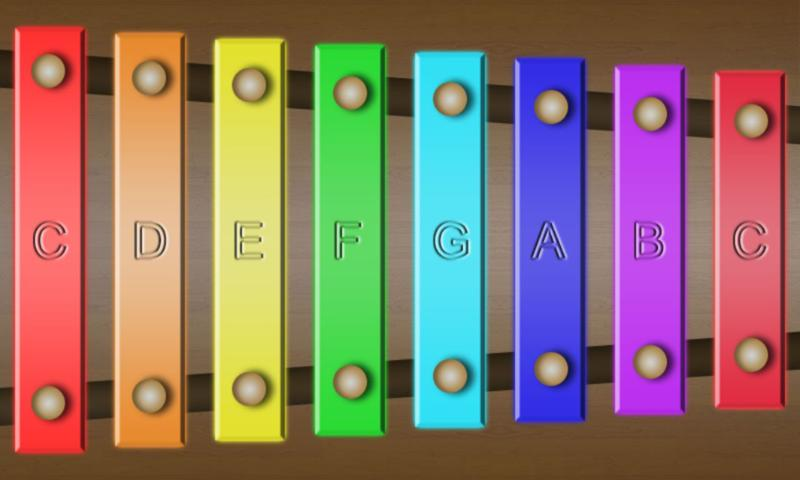
\includegraphics[width=0.36\linewidth]{bar_wrong_ph1.jpeg}
	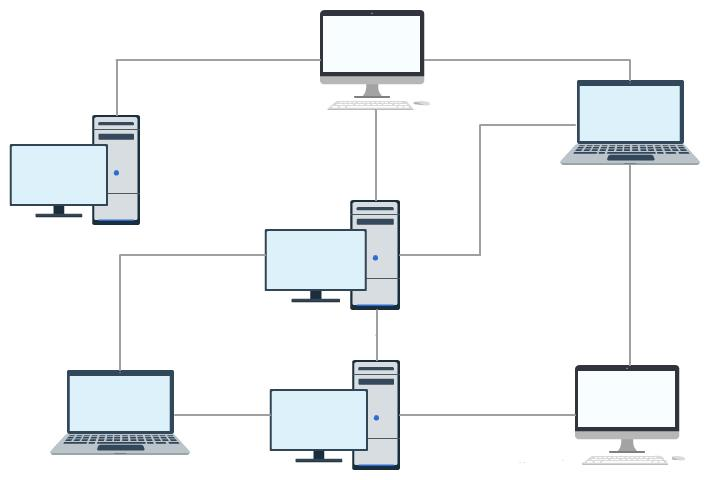
\includegraphics[width=0.36\linewidth]{box_wrong_ph1.jpeg}
	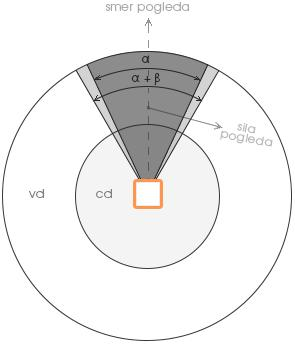
\includegraphics[width=0.24\linewidth]{pie_wrong_ph1.jpeg}
	\caption{\textbf{Images that were incorrectly classified as plots.} From left to right we can see images classified as bar plot, box plot and pie chart. None of them is a plot, but if we think in the context of CNNs, we can understand why the model made those mistakes.}
	\label{wrong phase1}
\end{figure}

We iterated through two more phases where we added corrected wrongly classified plots, to gather more hard examples for our training set.
We chose the final model based on best validation loss and used it to filter the extracted images from FRI, FMF and EF final theses. To additionally lower the false positive rates for each plot type, we only chose plots for which the model returned more than $99\%$ probability. Because we had enough plots, we could afford a more strict filter to reduce the number of false positives in each plot type class (images that do not belong to that plot type).

%-----------------------------------------------
%\section*{Further work}
%SAM PUSTIM TLE CE SE KEJ POMAGA
%Now we are trying to figure out, what are the attributes which define whether a plot is good or not. For determining the most popular attributes, we have decided to design some questionnaires and give it to a few people. On those questionnaires will be different plots. For each pair, an individual will decide which one is better and why. For instance \emph{"left plot is better because it uses appropriate colors", "right one is better because the axis are labeled",} ... When we will get the results from several questionnaires, we will gather the results and figure out what are the most important attributes to consider when evaluating the quality of plots. Next, we will use Amazon's Mechanical Turk to evaluate our plots data set. Workers will be asked similar questions, but now on attributes we have gathered from questionnaires. The plan is to evaluate pairs of pictures, for each which one has better \emph{attribute1, attribute2, ...} After we will have all the data, we are going to build a regression model that will predict how good the plot is and what are the values of its attributes -- those should explain why the plot is good/bad.


\section*{Surveys}
% Najprje smo nardil prvi vprašalnik, na podlagi tega pol MT, kako je ta zgledal..slika?.. kako smo generirali primerjave. Zakaj smo zbral na koncu samo lineplote?

% Our goal is to determine the aesthetic quality of a plot. Aesthetic quality is not well defined, so we measure it indirectly using a questionnaire based on pairwise comparisons and utilized Amazon's Mechanical Turk (MT). We developed the questionnaire with a test questionnaire with 10 plot comparisons, where the respondent had to choose a plot, combined with a cognitive interview, where the respondent had to explain what their decision was based on. We applied the questionnaire an opportunity sample of 10 1st year Master's students and our advisors. Based on the test data, we identified 5 key aspects: legend, color, axes, element sizing and readability. The final \href{LINK}{questionnaire} was composed out of pairwise comparisons of aesthetic quality and pairwise comparisons in each of these 5 key aspects.



Our goal is to determine the aesthetic quality of a plot. Since it is not well defined, we measure it using a questionnaire based on pairwise comparisons and utilize Amazon's Mechanical Turk (MT). We developed a test questionnaire with 10 plot comparisons, where respondents had to choose a plot and explain what their decision was based on. The questionnaire was answered by an opportunity sample of 10 1st year Master's students and our advisors. Based on the results, we identified 5 key aspects: legend, color, axes, element sizing and readability. The final \href{https://github.com/AndrejHafner/how-good-is-my-plot/blob/master/src/figures/questionnaire.png}{questionnaire} was composed out of 10 pairwise comparisons of aesthetic quality and pairwise comparisons in each of the 5 key aspects.

To estimate the time required for a pairwise comparison and determine the budget, we performed a test run on MT. The estimated time was one minute and the estimated cost 0.08\$. This cost was prohibitive for our budget, so we limited our analysis to line plots, that were the most common in the final theses.

We used the Swiss-system tournament for selecting the plot comparisons for surveys deployed on MT. After each survey was done, we gathered the results and counted how many wins each plot has so far. Based on the number of wins, we grouped the plots with the same number of points, and created plot comparisons for the next round of the tournament. We made sure that none of the comparisons were made more than once during all rounds. There were 9 rounds in the tournament, which is roughly equal to the logarithm of the plots in the dataset.

\section*{Plot quality prediction}
Our first approach was to generate embeddings from plots that were labeled by MT workers, and use traditional machine learning models to predict quality from them, and the second one was to fine-tune a CNN to directly output the quality. For target variable that described the quality of plots, we generated ELO ratings from the outcomes of the tournament that was played on MT.

\subsection*{ELO ratings}
The main goal of ELO ratings is to get a ranking of our dataset plots from their pairwise comparisons. The ratings represent latent strengths of our objects, and tell us relative quality of the plot, when compared with other plots from our dataset. Their advantage over the quality measured only by counting each plot's wins is that they also account for the quality of the opponent plot - the win counts more, if the opponent is a plot of high quality.
These ratings tell us the probability that plot 2 is chosen as better over plot 1:
$$ P(2\text{ is better than }1) = \dfrac{1}{1 + e^{x_1 - x_2}}, $$
where $x_1$ and $x_2$ are ELO ratings of the competing plots.
We inferred the model parameters $x_i$ using maximum likelihood. The solution is invariant to translation of latent strengths. To ensure model parameter identifiability, we fixed, without loss of generality, $x_1 = 0$. For the model to converge, we also needed to derive the gradient of the log-loss that we were minimizing using \emph{L-BFGS-B} method.
From this procedure we generated our target variable where the worst plot that didn't achieve any wins had rating of $-86$ and the best plot, that won all the comparisons, had rating of 109.

\subsection*{Prediction from embeddings}
We decided that since our data are images with complicated shapes, we need CNNs to get good features from them. That is why even for predictions with traditional models, we first extracted embeddings with ResNet101, and then continued with other approaches. We extracted embeddings with two different networks, first with the one pretrained only on ImageNet dataset, and the second one was the network that was finetuned for plot type classification.
% We hoped that that one will extract more information that is important
Embeddings were extracted from the last average pool layer and flattened, so we got a vector with 2048 features.
Since most of the learners don't do well with such a number of features, we decided to design our model as a pipeline, that will first transform the features with PCA and then train the selected models on features of lower dimension.

We split the data on train in test set as 80:20 and performed 5-fold grid search CV on the train set to select the hyper-parameters of the models.
For each model the number of principal components was selected based on the percentage of explained variance, which was one of the hyper-parameters.
The parameters that proved best after grid search CV are the following (for ImageNet embeddings / for embeddings from fine-tuned CNN):
SVR -- polynomial kernel of degree 1, 0.6 of explained variance / degree 1, 0.9 variance; Bayesian ridge regression -- 0.6 / 0.5 of explained variance; Random forest -- 2 minimal samples split, 500 estimators, 0.6 variance / 4 minimal samples split, 100 estimators, 0.9 variance; KNN -- 10 nearest neighbours and 0.9 variance / 10 neighbours and 0.8 variance.

\subsection*{Prediction with CNN}
The second approach to predict the plot quality (ELO ratings) from plot images was to fine-tune a CNN on the dataset. We used the same network as mentioned at plot type classification, we only adapted it for regression. The loss that we are optimizing was changed to MSE and the number of neurons in the last layer to 1.
We used the same train set as we used for other models, and again performed a 5-fold cross validation to select the best training parameters. In each split we took $10\%$ of the training set for validation, and with it we decided which model to chose - from which epoch, so that we didn't need to adapt this parameter. The parameters that we wanted to set with CV were learning rate, regularization parameter and batch size. The best MSE was achieved with learning rate $10^{-6}$, regularization $10^{-5}$ and batch size 50.

\section*{Results}
In this section we first present the results of plot type classification that was used for filtering the images, scrapped from theses. We continue with the results of plot quality prediction on the dataset obtained from MT. Finally, we analyze the subcategories results, which were not directly used in the plot quality prediction models, but can lead to some interesting findings.

\subsection*{Results of plot type classification}
We trained the classification model to minimize the log-loss, but that was just a surrogate loss we used to be able to train the network. The error that will more precisely estimate how well does the model perform based on our needs, is the number of false positives in each category. If we have enough plots extracted (or if the number of plots that we missed is sufficiently low), then we are only interested in the false positives of each plot type, as this are the images that we will need to manually remove.
From the final works our model filtered 8520 line plots, 4883 bar plots, 1799 scatter plots, 1259 pie charts, 1201 histograms, 288 box plots and 101 violin plots. For evaluation we sampled 1200 plots from line and bar plots, because there were too many of them and for others we manually checked all plots. There were 18 false positives in line plots, 3 in bar plots, 76 in scatter plots, 13 in pie charts, 100 in histograms, 90 in box plots and 91 in violin plots. To see how many plots we missed, we sampled 500 images from all images that were not included in the above categories. In that sample there were only 3 plots.

\subsection*{Results of quality prediction}
In table \ref{table_of_results} we can see the results of some of the models with which we tried to predict plot quality. We can see that none of the predictors achieved much better results than the one that was predicting the mean value of the target variable in train dataset. The best of them is Bayesian Ridge Regression, but from the small improvement compared to the mean predictor, we can't say that it could be of any use. We will further discuss what could be the reason for the models to not be able to give good predictions in the next section.

\begin{table} \centering
\begin{tabular}{|c|c|c|c|}
    \hline
     Data & Model & Mean & Std  \\
     \hline
     \hline
     train elo & Mean predictor & 188 & 100 \\
     \hline
     emb & SVR & 188 & 102 \\
     \textbf{emb} & \textbf{Bayesian Ridge} & \textbf{183} & \textbf{98} \\
     emb & Random Forest & 188 & 100 \\
     emb & KNN & 187 & 98 \\
     \hline
     emb. ft & SVR & 191 & 104 \\
     emb. ft & Bayesian Ridge & 192 & 103 \\
     emb. ft & Random Forest & 189 & 96 \\
     emb. ft & KNN & 216 & 103  \\
     \hline
     images & finetuned ResNet101 & 186 & 99 \\
    \hline
\end{tabular}
     \caption{Results of prediction models on the test set. In the table we can see the data that was used to train the models and the mean and standard deviation of the estimate (MSE) on all test datapoints.}
     \label{table_of_results}
\end{table}

\subsection*{Analysis of subcategories}
To analyze which categories are more important in the decision, we shared one point among the categories that were considered in each comparison (if there were three categories considered, each of them scored one third of the point).
On the figure \ref{categories_count} we can see the count of points over all matches for the winning and for the losing plot. As expected, the number of points given to the winning plot is higher, but still we can see that the losing plots were often better in some of the categories. The correlation that is written above bars was calculated between the vector of wins (-1 if first plot won and 1 if second) and the vector of each category: $-\frac{1}{n}$ if the first plot was chosen as better in this category, 0 if the category was not considered and $\frac{1}{n}$ if the second plot chosen -- $n$ being the number of categories considered in this comparison.
Based on the workers answers, readability is the most important quality. It was also the most often selected category for the winning plot and the least often for the losing plot.
The correlation between the categories is low (the highest being $0.23$ between readability and legend), therefore we can conclude that these are independent attributes of the plots.

We also checked if there exist plot comparisons, where the plot chosen as worse overall, was better at more attributes than the winning plot. After analysing 273 cases where that happened, the attribute that was the most often selected as better for winning plot in these cases was again readability. This means that the workers considered it more important then those that were chosen as better for the losing plot.
% So for instance, if one plot had better legend, colors and axes, but the other has better readability, the second one was chosen to be best.

\begin{figure}
	\includegraphics[width=\linewidth]{categories.png}
	\caption{On this figure we can see how many points were given for each category to the winning and to the losing plot. The categories are sorted based on the correlation between each category and the win of the plot, that is also annotated at the top of the bars.}
	\label{categories_count}
\end{figure}


%------------------------------------------------

\section*{Discussion}
The model that we build for the classification between plot types proved useful for gathering big dataset of plots. It has a low number of missed plots, and for most of the categories low false positive rate. We wouldn't recommend it if you are interested in violin and box plots. The reason it works bad for those is probably low number of training examples. We should be aware that this model is build based on the iterations over the plots from final thesis of FRI, FE and FMF, and also the negative images came from the same source. Therefore this model works well for our purpose, but could be much worse if it was used out of this context. The evaluation is negatively biased because some of the images that we evaluated it on are also in the training set - because of iterative training. If it were used for plots that came from different source we would probably need to additionally fine-tune it.

The most important question is, why did our model fail at quality prediction? One of possible problems is the number of plots that were taken into account and therefore also the number of unique workers that scored the plots. Main goal of the project was to get what people notice when they look at a plot and what attracts them, but there is no single definition of what a quality plot is. We like different things and therefore our opinions about visual aspects of plots are different. To get a general opinion, we would need more data. The same problem arises in the fine-tuning of the CNN. The plots in our dataset have many differences, so for the network to learn that the differences that are important for final ratings lie in the legend, or readability (if our hypothesis that those are important for the quality even holds), we would need a lot more training examples from which the network could learn.

From the subcategories analysis we can see that the most important thing that people notice when they are visually comparing the plots, is their readability. The least important is the sizing of the elements and the color of the plots. We should take that into account when generating new plots and ensure that they are clear and readable.

%------------------------------------------------

\section*{Acknowledgments}
The authors would like to thank mentors assoc. prof. dr. Erik Štrumbelj and assoc. prof. dr. Tomaž Curk for their guidance and ideas, which helped solve many problems that arose during the research process.

%----------------------------------------------------------------------------------------
%	REFERENCE LIST
%----------------------------------------------------------------------------------------
\bibliographystyle{unsrt}
\bibliography{report}
\end{document}